\ps{We could include a lot more plots in here if we want, things like trace and corner plots for the
	3 fits could go in here, also have remnant fraction plots that might be interesting to compare.}


\begin{figure}
	\begin{center}
		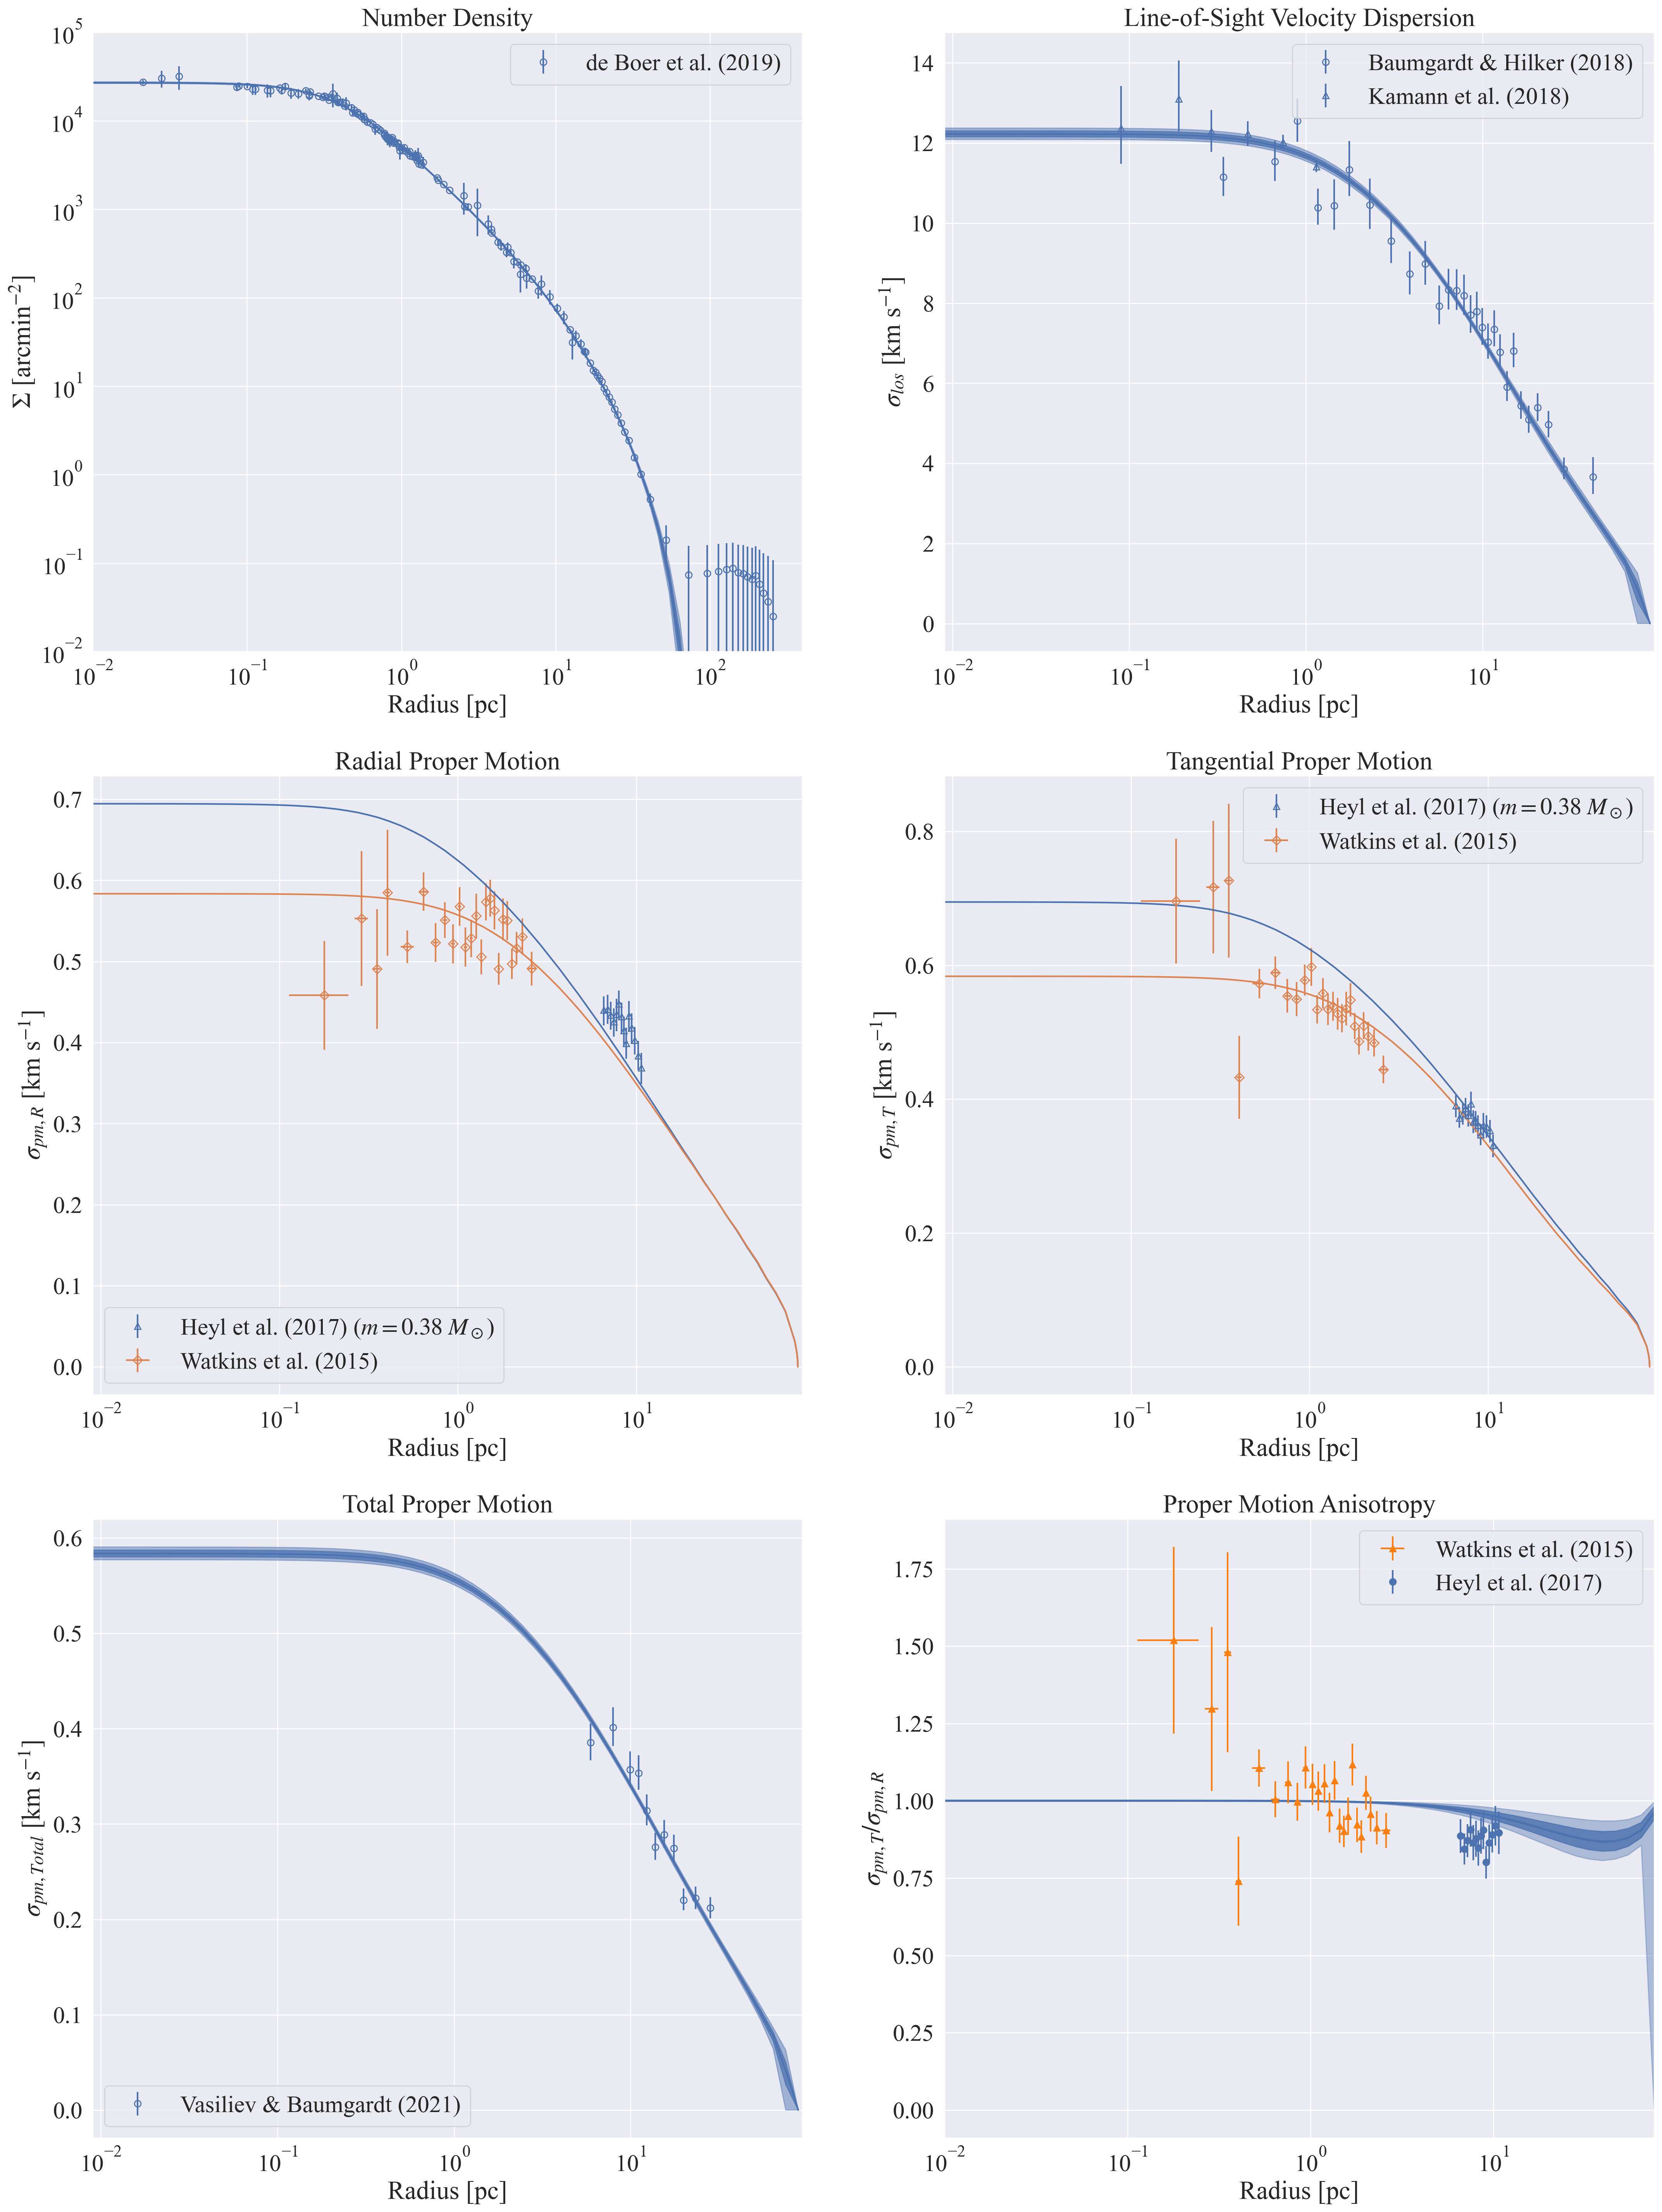
\includegraphics[width=0.9\textwidth]{figures/prev_nobin/obs_panel.png}
	\end{center}
	\caption{Model fits to the observables for models with no binary stars.}
	\label{fig:nobin_obs_panel}
\end{figure}

\begin{figure}
	\begin{center}
		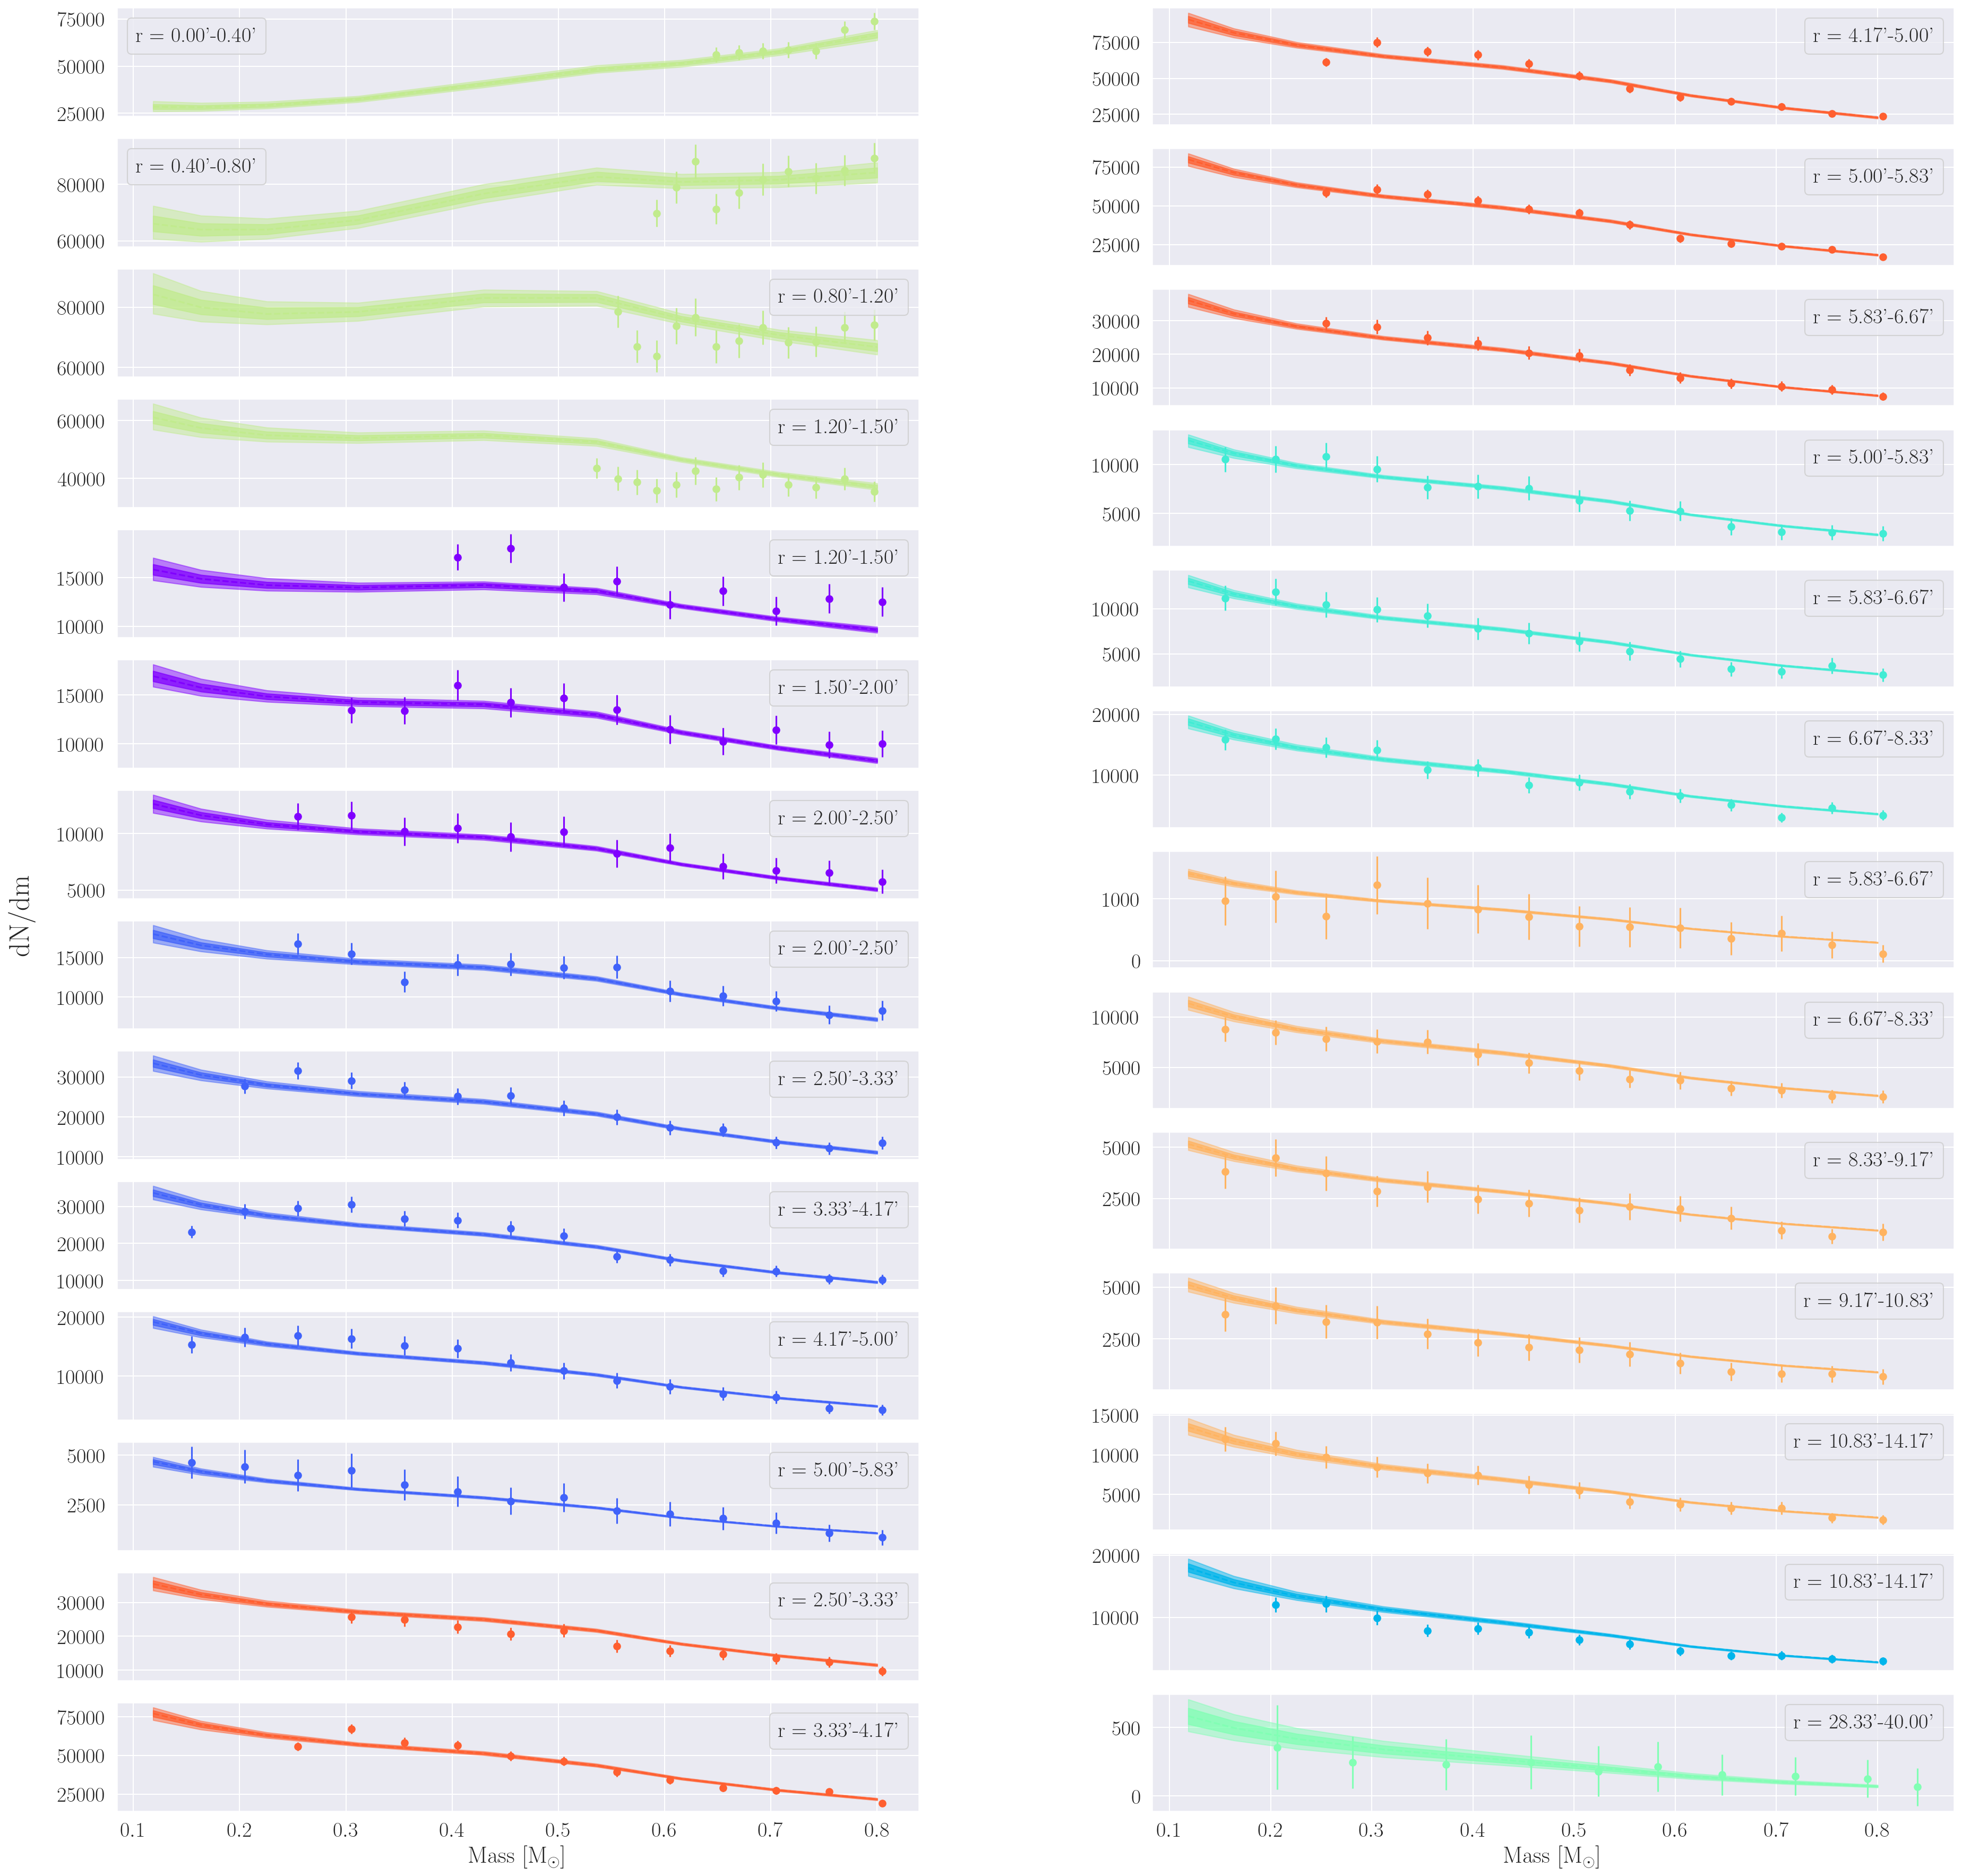
\includegraphics[width=0.9\textwidth]{figures/prev_nobin/mass_fun.png}
	\end{center}
	\caption{Model fits to stellar mass function data for models with no binary stars.}
	\label{fig:nobin_mass_fun}
\end{figure}

\begin{figure}
	\centering
	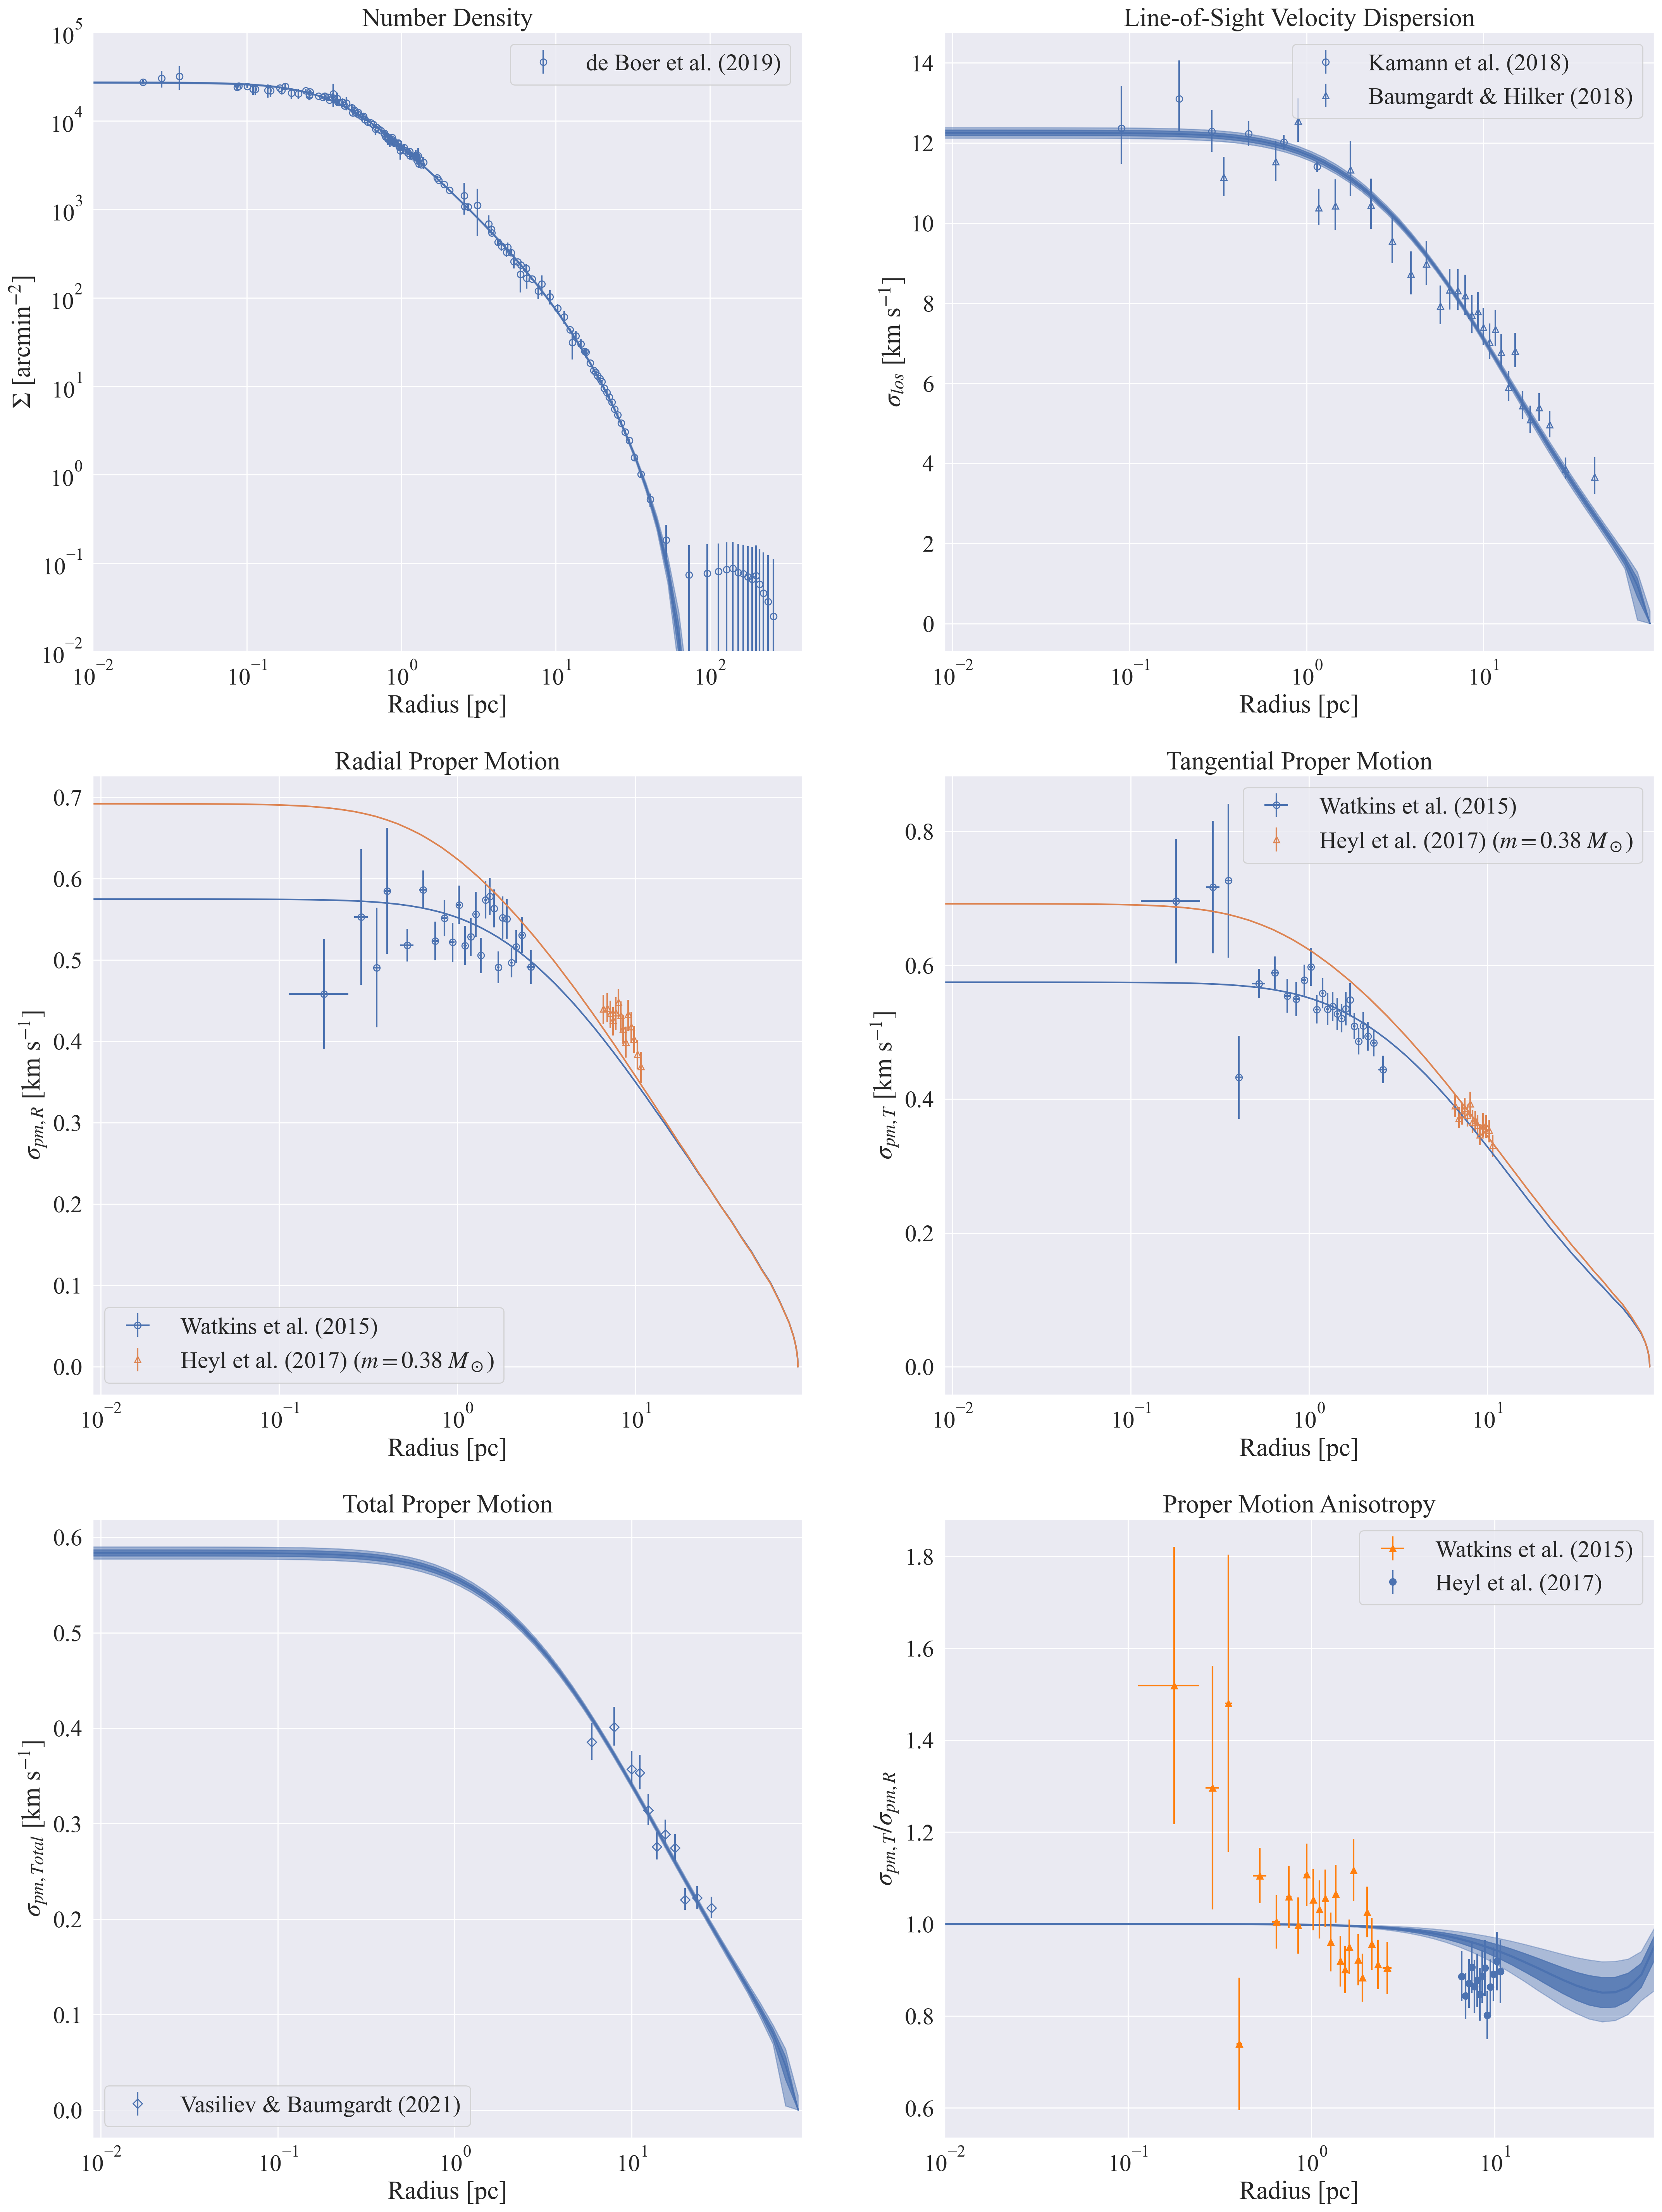
\includegraphics[width=0.8\textwidth]{figures/high_bin_model/obs_panel.png}
	\caption{Model fits to the observables for models with a $10\%$ binary fraction.}
	\label{fig:highbin_obs_panel}
\end{figure}


\begin{figure}
	\centering
	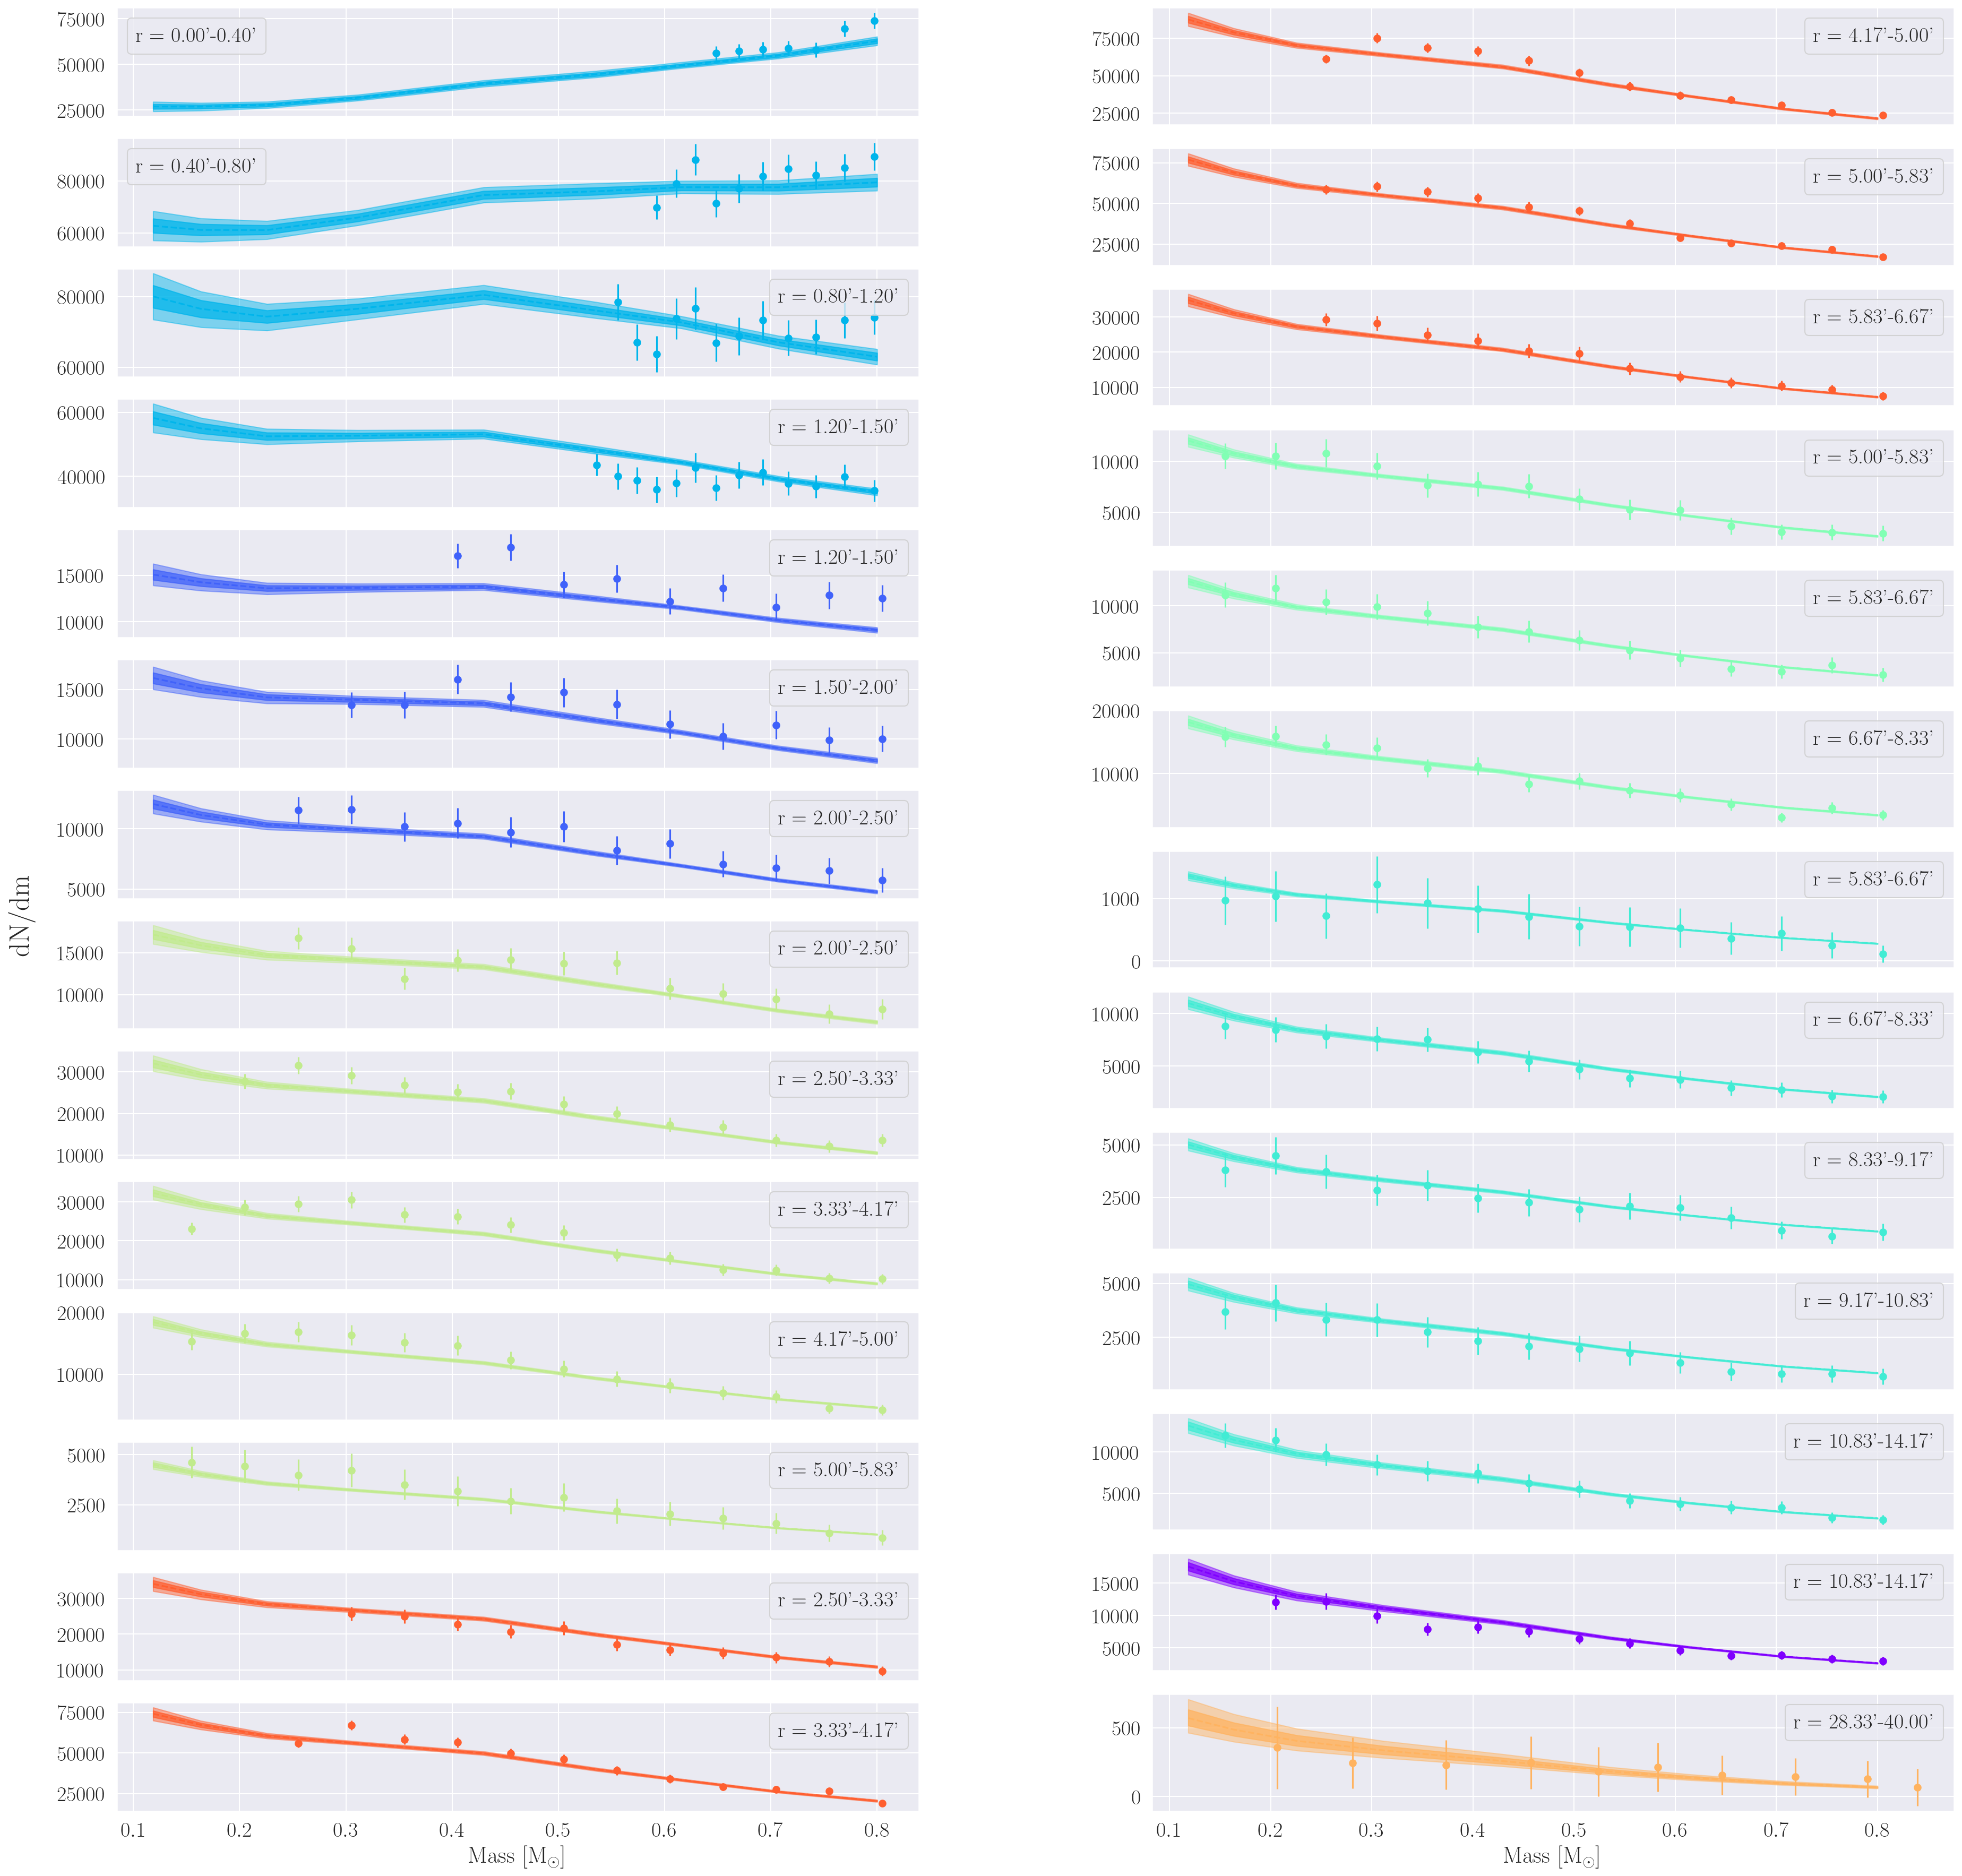
\includegraphics[width=0.8\textwidth]{figures/high_bin_model/mass_fun.png}
	\caption{Model fits to the stellar mass function data for models with a $10\%$ binary fraction.}
	\label{fig:highbin_mass_fun}
\end{figure}